\documentclass[12pt,a4paper]{report}
\usepackage[T1]{fontenc}
\usepackage[utf8]{inputenc}
\usepackage[brazilian]{babel}
\usepackage{amsmath}
\usepackage{graphicx}

\renewcommand\thesection{\arabic{section}}

\author{\textbf{
 Eduardo Delgado Bier
 Fernanda de Camargo Magano 
 Florence Alyssa Sakuma Shibata 
 Shayenne da Luz Moura 
 Théo Dury }}
\title{\textbf{Fase 1 - Documento de Requisitos do sistema}}
\date{outubro de 2015}

\begin{document}


% capa
\begin{titlepage}

\begin{center}
{\large IME-USP}\\[0.2cm]
{\large Trabalho de Engenharia de Software}\\[5.1cm]
{\bf \huge Fase 1 - Documento de Requisitos do sistema}\\[5.1cm]
\end{center}


\begin{flushright}

 Eduardo Delgado Bier \\
 Fernanda de Camargo Magano \\
 Florence Alyssa Sakuma Shibata \\
 Shayenne da Luz Moura \\
 Théo Dury \\
 
\end{flushright}

\begin{center}
{\large \textbf{São Paulo}}\\[0.2cm]
{\large \textbf{2015}} \\[0.2cm]
\end{center}

\end{titlepage}

\tableofcontents

\newpage

\section{Introdução}

\subsection{Objetivos deste software}

Quando uma pessoa decide tratar algum problema de saúde ou algo similar em um hospital, geralmente seus dados ficam restritos somente àquela unidade ou à sua rede hospitalar. Caso o hospital reconheça que o tratamento em sua unidade não é possível ou algum paciente tenha pretensões de continuar seu tratamento em algum lugar, cabe ao paciente levar consigo suas informações a respeito do diagnóstico e o tratamento a que foi submetido.
Visando a evitar o trabalho de transporte de informações de forma manual, o desperdício de tempo e de recursos, perda de informações e possíveis ambiguidades em suas interpretações, o sistema a ser desenvolvido neste projeto consiste na unificação de dados hospitalares em relação aos dados dos pacientes: ao diagnóstico, processo do tratamento, medicamentos indicados, estado atual do paciente, etc.

\textbf{Público Alvo:} esse software se destina, principalmente, aos médicos para terem acesso e poder modificar prontuários de paciente. Também é extretamente útil para os pacientes, pois podem acompanhar todo seu histórico de medicamentos, exames e consultas.



\subsection{Escopo do produto}

\subsubsection{Nome do produto e seus componentes}
IMECare:

\begin{itemize}
\item Organização de prontuários de pacientes
\item Fácil acesso às informações pelos médicos, enfermeiros e pacientes
\item Dados disponíveis na web, de modo que qualquer hospital integrado ao sistema tenha acesso
\item Garante praticidade e evita perda de informações importantes 
\end{itemize}


\subsubsection{Descrição do produto}

O produto será utilizado por hospitais e pacientes dos mesmos. Eles terão acesso a uma interface web (pretendemos utilizar um site) e por meio dela conseguirá acessar dados, modificar, checar os agendamentos e realizar alterações de datas, quando desejar.



\subsubsection{Missão do produto}

\begin{itemize}

\item Economizar tempo, já que com o histórico unificado dos pacientes, o médico já saberá qual é situação de todo o processo a que o paciente foi submetido;
\item Apresentar visão panorâmica do histórico e evolução do paciente;
\item Como consequência, pode-se utilizar os dados fornecidos por esse projeto para garantir um direcionamento na gestão de serviços de atendimento às pessoas doentes, permitindo organização por parte de quem trabalha nos hospitais. Assim, ocorre melhoria na qualidade do serviço e permite economia de tempo.

\end{itemize}




\subsection{Siglas e definições}

\textbf{SGBD} - Sistema Gerenciador de Banco de Dados \\
\textbf{RG}   - Registro Geral\\
\textbf{CPF}  - Cadastro de Pessoa Física\\



\section{Descrição geral do produto (na visão dos usuários)}

\subsection{Perspectiva} 

Diagramas de caso de uso:

\begin{figure}[h!]
  \caption{Caso de uso- Médico}
  \centering
  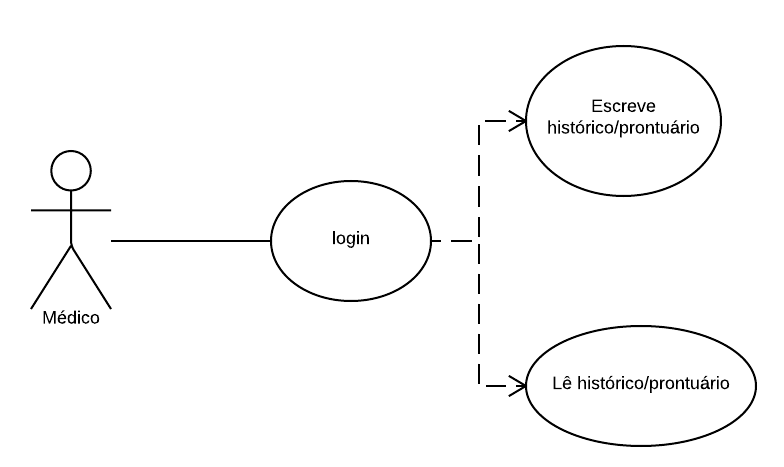
\includegraphics[scale=.5]{doctor.png}
\end{figure}

\begin{figure}[h!]
  \caption{Caso de uso- Enfermeiro}
  \centering
  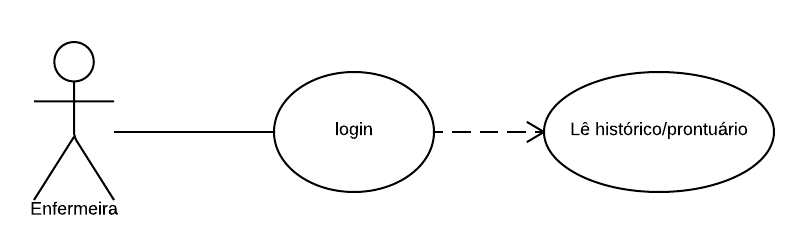
\includegraphics[scale=.5]{nurse.png}
\end{figure}

\begin{figure}[h!]
  \caption{Caso de uso- Paciente}
  \centering
  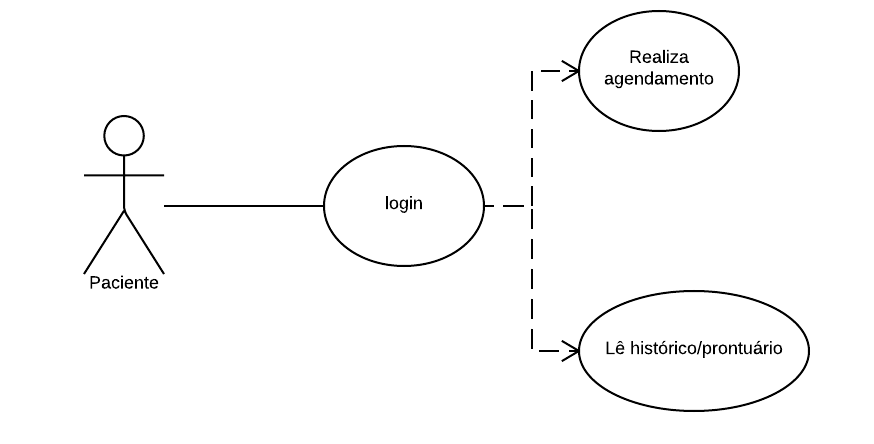
\includegraphics[scale=.5]{patient.png}
\end{figure}

\begin{figure}[h!]
  \caption{Caso de uso- Secretária}
  \centering
  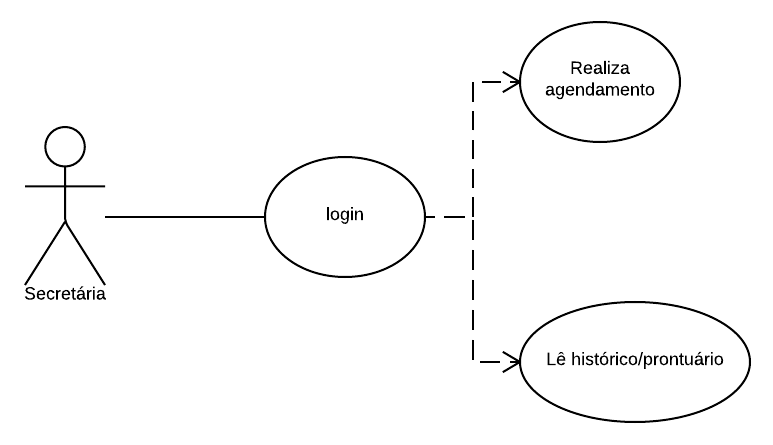
\includegraphics[scale=.5]{secretary.png}
\end{figure}


\newpage

\subsection{Usuários do sistema}

\begin{itemize}
\item Pacientes: podem acessar suas informações presentes no sistema e agendar/reagendar consultas
\item Médicos: acessam/alteram os prontuários dos pacientes
\item Enfermeiros: consultam informações dos prontuários dos pacientes
\item Secretários: responsáveis pelo agendamento de consultas

\end{itemize}




\section{Requisitos específicos}


\subsection{Identificação dos requisitos}

\subsection{Prioridades dos requisitos}

Como o projeto é grande, é necessário ter um planejamento e analisar o que é mais prioritário dentre as tarefas que precisam ser realizadas. Abaixo, estão definidos o que significa ser: essencial, importante ou desejável. \\

\begin{itemize}
\item \textbf{Essencial:}
É o requisito sem o qual o sistema não entra em funcionamento.
São extremamente necessários, não podem ser adiados ou feitos parcialmente.

\item \textbf{Importante:}
Sem os requisitos importantes, o sistema até consegue entrar em funcionamento, mas não de forma satisfatória. São requisitos que devem ser implementados, mas se não forem, ainda é possível ter o sistema em funcionamento.


\item \textbf{Desejável:}
É o requisito que não compromete as funcionalidades básicas do sistema. 
Podem ser deixados para versões posteriores do sistema, se não der tempo de ser concretizado na fase inicial.


\end{itemize}


\subsection{Descrição dos requisitos}

\begin{itemize}
\item \textbf{Gerenciamento dos pacientes}

O sistema precisa prover uma forma dos pacientes se cadastrarem no sistema e acessarem seus dados quando fizerem login.\\
\\ Os pacientes têm cpf, rg, contato (seja telefone/ endereço), tipo sanguíneo.
Um paciente pode ter uma ou mais doenças associadas a ele. Cada doença vai gerar um determinado grupo de exames pedidos. Um mesmo exame pode ser pedido para problemas de saúde diferentes e podem ser feitos em laboratórios diferentes.\\
Uma maneira encontrada de armazenar os dados do paciente de forma a conter seu histórico de consultas, exames e informações em geral, foi criar um prontuário que conterá um conjunto de registros sobre os mais diversos conteúdos relacionados ao paciente. 
Assim, tudo isso poderá ser visto através do prontuário do paciente que está consultando o sistema. \\
Além disso, o sistema deve possibilitar consultar quais serão as datas/horários das próximas consultas e, além disso, permitir alteração das datas (caso o paciente deseje e os médicos tenham aqueles dias disponíveis para atendimento).

\item \textbf{Gerenciamento dos funcionários}

Como funcionários o sistema terá: médicos, enfermeiros e secretários.
Eles têm cpf, rg, contato (seja telefone/ endereço), unidade(s) em que trabalham, já que o sistema integra mais de um hospital.
No caso do médico, outro atributo é a especialidade em que trabalha.

Os médicos devem poder acessar o sistema, consultar e modificar dados dos pacientes. \\
Quando ocorre uma consulta, o médico pode realizar diagnóstico, fazer prescrições e/o analisar os exames. Com base nisso, o médico receita medicamentos numa determinada dose. Os medicamentos podem trazer uma melhoria no quadro do paciente ou não surtirem muito efeito. Isso deve ser registrado, pois pode haver troca do medicamento. Assim, os médicos devem adicionar registros ao prontuário do paciente quando houver alguma consulta. \\


Os enfermeiros podem apenas consultar informações dos pacientes em que atende. \\
Os secretários são responsáveis pela parte de agendamento das consultas.

\end{itemize}



\subsection{Requisitos Funcionais}

\begin{center}
\textbf{=======================\\
Descrição dos Use Cases\\
=======================\\}
\end{center}

\subsubsection{<<<<<<Caso de uso: Realiza Agendamento>>>>>>} 

\textbf{Ator primário:} Paciente \newline

\textbf{Objetivo no contexto:} Marcar um horário para consultar um médico de alguma de especialidade. Ele pode cancelar e remarcar consultas já agendadas.\newline

\textbf{Pré-condições:}  O usuário e senha do paciente precisam ser válidos. O sistema deve possuir o cadastro do paciente para permitir o seu acesso.\newline

\textbf{Trigger:} O usuário decide consultar informações sobre seu agendamento.\newline


\textbf{Cenário:}
\begin{enumerate}

\item O paciente entra na página linux.ime.usp.br/~imecare
\item O paciente digita sua identificação e senha (com pelo menos 6 caracteres, sendo pelo menos um deles um caracter especial)
\item O sistema apresenta um menu para o paciente escolher a função que deseja executar.
\item O paciente seleciona o botão "Agendamento"
\item O sistema apresenta uma lista das consultas já marcadas nos últimos 12 meses e um menu com opções "Marcar consulta", "Alterar consulta", "Cancelar consulta".
\item O paciente seleciona o botão "Marcar consulta". 
\item O sistema apresenta um formulário para o paciente escolher o hospital, a especialidade, o médico e a data desejada. O resultado pode ser reordenado por médico ou data.
\item O paciente escolhe dentre as datas, uma que deseje. 
\item O sistema registra a opção selecionada como uma consulta marcada. Retorna resultado (sucesso, falha).
\item O paciente seleciona o botão "Alterar consulta".
\item O sistema apresenta as próximas consultas e permite selecionar a que se deseja alterar.
\item O paciente seleciona a consulta.
\item O sistema apresenta a disponibilidade dos médicos e seus respectivos horários.
\item O paciente pode selecionar uma das opções.
\item O sistema registra a consulta e retorna o resultado (sucesso, falha)
\item O paciente seleciona o botão "Cancelar consulta".
\item O sistema apresenta as próximas consultas e permite selecionar a que se deseja cancelar.
\item O paciente seleciona a consulta.
\item O sistema cancela a consulta e retorna o resultado (sucesso, falha)

\end{enumerate}

\textbf{Exceções:}
1. Se a identificação e a senha não estiverem corretas, olhe o use case de Validação.\newline


\textbf{Prioridade:} Prioridade moderada, pode ser implementado depois das funções básicas.\newline

\textbf{Quando estará disponível:} Segundo incremento\newline

\textbf{Frequência de uso:} Alta frequência\newline

\textbf{Canal para o ator:} Web site\newline

\textbf{Questões abertas:}
\begin{enumerate}
\item O que acontece quando dois pacientes tentam marcar uma mesma data e horário ao mesmo tempo?
\item O que acontece em caso de queda ou falha ao marcar o agendamento?
\end{enumerate}



\subsubsection{<<<<<<Caso de Uso: Validação>>>>>>}

\textbf{Atores:} paciente, médico, secretário, enfermeiro\\

\textbf{Objetivo no contexto:} Validar o acesso ao sistema.\\

\textbf{Pré-condições:} O ator deve possuir um cadastro no sistema.\\

\textbf{Trigger:} O ator decide consultar o sistema\\

\textbf{Cenário:}
\begin{enumerate}
\item O ator entra na página linux.ime.usp.br/~imecare
\item O sistema apresenta um formulário para que o ator entre com sua identificação e senha.
\item O ator digita seus dados.
\item O sistema verifica se os dados são consistentes com o que há no banco de dados.
\item Caso os dados sejam consistentes, a interação entre o usuário e o sistema é liberada.
\item Caso contrário, o sistema devolve erro e volta para o segundo item.
\end{enumerate}



\textbf{Prioridade:} Alta prioridade\\

\textbf{Quando estará disponível:} Primeiro incremento\\

\textbf{Frequência de uso:} Alta frequência\\

\textbf{Canal para o ator:} Web site\\

\textbf{Questões abertas:}
\begin{enumerate}
\item O que acontece quando o ator tenta logar no sistema por várias vezes sem sucesso?
\item Haverá algum sistema de recuperação de identificação/senha?\\
\end{enumerate}



\subsubsection{<<<<<<Caso de Uso: Leitura de prontuário>>>>>>}

\textbf{Ator primário:} médico, enfermeiro e secretário\\

\textbf{Objetivo no contexto:} Ler as informações contidas no prontuário de um paciente.\\

\textbf{Pré-condições:} Estar logado no sistema e o paciente possuir um prontuário no sistema.\\

\textbf{Trigger:} Necessidade de recuperar informações sobre determinado paciente\\

\textbf{Cenário:}
\begin{enumerate}
\item Ver caso de validação
\item No site, terá um campo de busca por um paciente onde o ator deverá inserir o identificador do paciente.
\item O sistema mostra o resultado na tela.

\end{enumerate}

\textbf{Exceções:}
1. Prontuário inexistente.\\

\textbf{Prioridade:} Alta\\

\textbf{Quando estará disponível:} Segunda incrementação\\

\textbf{Frequência de uso:} Alta\\

\textbf{Canal para o ator:} Website\\


\subsubsection{<<<<<<<<Caso de Uso: Escrita de prontuário>>>>>>}

\textbf{Ator primário:} médico, enfermeiro e secretário\\

\textbf{Objetivo no contexto:} Ler as informações contidas no prontuário de um paciente.\\

\textbf{Pré-condições:} Estar logado no sistema e o paciente possuir um prontuário no sistema.\\

\textbf{Trigger:} Necessidade de recuperar informações sobre determinado paciente\\

\textbf{Cenário:}
\begin{enumerate}
\item Ver caso de validação
\item No site, terá um campo de busca por um paciente onde o ator deverá inserir o identificador do paciente.
\item O sistema mostra o resultado na tela e os campos de edição.
\end{enumerate}


\textbf{Exceções:}
1. O médico tenta modificar um prontuário ao qual não tem acesso.\\

\textbf{Prioridade:} Alta\\

\textbf{Quando estará disponível:} Segunda incrementação\\

\textbf{Frequência de uso:} Alta\\

\textbf{Canal para o ator:} Website\\



\subsection{Requisitos não-funcionais}

\begin{itemize}

\item \textbf{Interface Amigável:} 

\textbf{Descrição:} O sistema deve apresentar uma interface intuitiva para os usuários do sistema, com menus e botões que facilitem a navegabilidade pelo sistema.
Além disso, ser user-friendly é importante, visto que o sistema não pode exigir conhecimentos avançados de informática. A integração de hospitais visa atender o público em geral e, portanto, tanto o vocabulário do site, quanto o modo de uso, não deve ser complexo. 

\textbf{Prioridade:} importante


\item \textbf{Sistema de Ajuda} 

\textbf{Descrição:} Um menu de ajuda é sempre interessante para que os usuários possam tirar suas dúvidas a respeito do uso do sistema, ou pelo menos uma página de FAQ. Contudo, o projeto é grande e essa funcionalidade pode ser deixada para futuras versões. 

\textbf{Prioridade:} Desejável \newline


\item \textbf{Restrições de acesso/modificação do sistema}

\textbf{Descrição:} Realiza o controle de acesso, restrições de que pode alterar os dados do sistema e está relacionado com a segurança da informação.

\textbf{Prioridade:} importante

\end{itemize}


\end{document}